\documentclass[doc, a4paper, apacite]{apa6}

\usepackage[american]{babel}

\usepackage{csquotes}
%\usepackage[style=apa,sortcites=true,sorting=nyt,backend=biber]{biblatex}
%\DeclareLanguageMapping{american}{american-apa}
\usepackage{threeparttable}
\usepackage{booktabs} % For nice tables
\usepackage{amsmath} % For \text{} function 
\usepackage{setspace}

\title{Looking at bumping up uncertainty and effects of background.}
\shorttitle{DSTL08}

\author{Charlotte E. R. Edmunds, Adam Harris, Magda Osman}
\affiliation{Queen Mary, UCL, University of London \\ 26 November 2020}

%\leftheader{Edmunds}

%\abstract{}
%
%\keywords{}

\begin{document}
\maketitle
\doublespacing

\section{Method}
\subsection{Participants}
Based on the previous experiment, we recruited 480 participants through Prolific Academic, 80 participants per condition. 
Due to the particulars of the task, we did not not recruit participants that are colour blind. 
Participants were paid \pounds1.50 for their participation. 

Exclusions will aim to remove those participants that are either bots or failed to concentrate. 
Participants will also be excluded if they fail to reach the criterion on the categorisation training task. 
If participants fail to successfully learn the categorisation task, they will not continue to the monitoring task and will not be paid for their time. 
This fact will be made explicit in the advert on Prolific Academic and in the consent form. 

\subsection{Materials}
This experiment was run online using JavaScript. 

\subsection{Design}
The experiment had a 3 (Uncertainty presentation: Control, Categorical, Uncertainty) by 2 (Background: Black, Radar) between-subjects design. 
Participants viewed one of the uncertainty presentation condition displayed on one of two background: either black as in Experiments DSTL02 and DSTL03 or black with a green radar-esque rings (as shown in Figure~\ref{fig:radar}). 

\begin{figure}
	\centering
	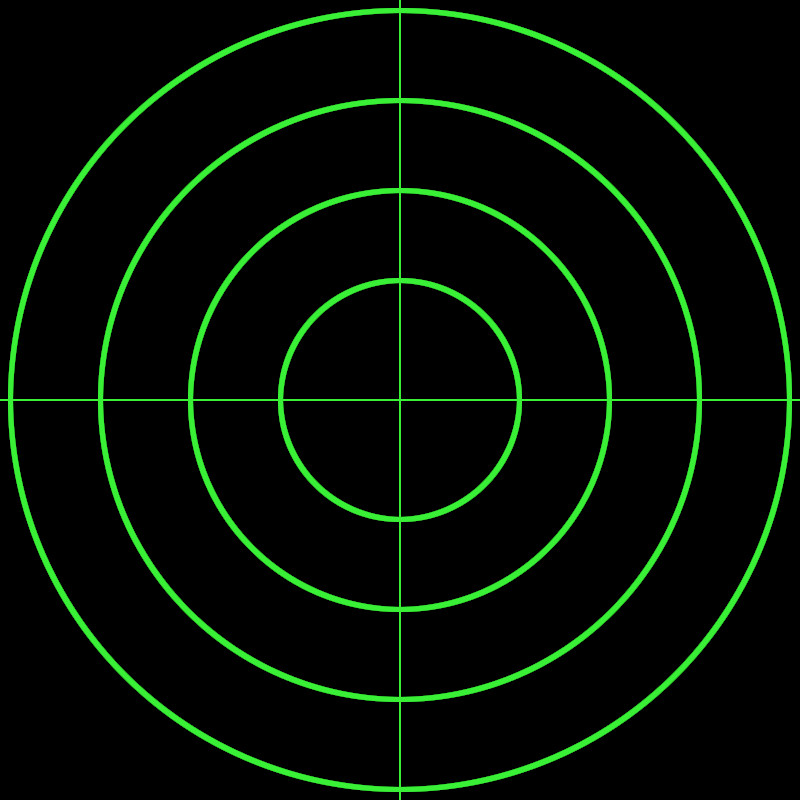
\includegraphics[width=0.5\textwidth]{images/radar.jpg}
	\caption{}
	\label{fig:radar}
\end{figure}

There were three types of uncertainty presentation:
\begin{enumerate}
	\item In the control condition, there will be four categories of entities: Unknown, Friendly, Hostile and Neutral.\\
	\item In the categorical condition, there will be six categories of entities: Unknown, Friendly, Assumed Friendly, Hostile, Assumed Hostile and Neutral. The Assumed- and Certain- versions of a categorisation (e.g. Friendly) will be different colours. 
	\item In the uncertainty condition, there will be six categories of entities: Unknown, Friendly, Assumed Friendly, Hostile, Assumed Hostile and Neutral. In this condition, the Assumed- and Certain- versions of a categorisation (e.g. Friendly) will be the same colour, where the Certain- version is a filled circle and the Assumed- version is unfilled. 
\end{enumerate}

\subsection{Stimuli}
The stimuli will be circles $30px$ in diameter. 
To mimic the displays found on Naval vessels, each circle will have a randomly generated six-digit alphanumeric code that floats next to it. 
Figure~\ref{fig:conditionColours} shows the colour mappings for the control conditions in the previous experiment and both colour way conditions in the current experiment. 

The entities will be circles that are either grey or one of five colours. 
The grey circle will have a brightness of 60\%, rgb(153, 153, 153). 
The colours will all be of equal saturation (60) and brightness (90). 
They will be presented in six colours: red (H360, rgb(230, 92, 92)), yellow (H72, rgb(202, 230, 92)), green (H144, rgb(92, 230, 147)), blue (H216, rgb(92, 147, 230)), and purple (H288, rgb(202, 92, 229)).

Across all conditions, Hostile will be red, Unknown yellow, Friendly green and Neutral blue. 
In the categorical condition, Assumed Friendly and Assumed Hostile will be randomly assigned to grey and purple. 
In the uncertainty condition, Assumed Friendly and Assumed Hostile will be an unfilled circle the same colour as Friendly and Hostile entities respectively. 

\subsection{Procedure}

The experiment presents coloured circles moving on a black background, $800px$ square. 
The experiment has two phases: categorisation training and the monitoring task.
The categorisation training phase remains unchanged from DSTL02.  

\subsubsection{Categorisation training}
In this section, participants will learn which colour is associated with which label. 
The instructions for this task are displayed below. 
On each trial, a single stimulus was shown, on a black background. 
The order of the stimuli shown was pseudo-randomised: for each block of four or six stimuli (depending on the condition) participants saw all the possible stimuli in a random order. 
Along the top of the screen, buttons were displayed showing the available options (either four or six depending on the condition). 
To respond participants clicked on the appropriate option and then received feedback for one second. 
If they respond correctly, the feedback read ``Correct'' in white plus a reinstatement of the correct answer in white e.g. ``It was a friendly craft.'' 
If they respond incorrectly, the feedback read ``Incorrect'' in white plus the correct answer in white e.g. ``It was a friendly craft.''
Compared to the first experiment, we made the feedback all white rather than prime people with the idea that green/red represents positive/negative results respectively.
Feedback will be displayed for 1500ms.
Between trials, there was blank screen shown for 500ms. 
The trial will time out after 5 seconds. 

This section will end either once 100 trials have been shown or once the participants have exceeded the learning criteria, whichever happens first. 
Participants pass the learning criteria if they achieved eight correct trials out of the last 10. 
If participants fail to reach the learning criteria within 100 trials, they will not proceed to the monitoring phase.
Participants who fail this stage will not be paid. 

\subsubsection{Monitoring task}
At the beginning of the experiment, 24 entities were (uniform) randomly placed in the box. 
To program movement, each entity will be associated with a coordinate within the viewing area or in a 50 pixels wide frame surrounding the viewing area. 
Entities move towards those points at a rate of 50 pixels per second.
The associated points change every 2000ms or if the entity reaches the point, whichever occurs first. 
At this point, for the x-coordinates, a number is sampled from a uniform distribution between 0 and 1.
If the sampled number is less than or equal to 0.33, the x coordinate will move to the left, if it is greater than or equal to 0.66 it will move to the right, otherwise the x-coordinate will remain the same. 
A similar sampling process occurred for the y-coordinate, but with up and down as appropriate. 

Entities were not allowed to collide and they will be able to ``wrap,'' i.e. an entity leaving the left portion of the screen will reappear on the right.
To prevent entities being half visible on opposite edges of the screen, there is an invisible border around the viewing window 50px wide, in which the stimulus can wrap. 

On most of the trials, one entity changed from one category/colour to another. 
On the remaining five trials in each within-subject condition, there will be no change of category/colour. 
The participants' task was to identify which entity changed, and click on that entity. 
Responses and reaction times were collected. 
There was a variable inter-trial interval. 
The trial time-outed if participants took more than five seconds to make a response. 

Additionally, participants were told that they are sharing this monitoring task with another trainee seaman called ``Smith.'' 
This was in order to provide a cover story for why they are unable to respond during the inter-trial interval. 
Participants will be notified whether it was their go or Smith's by a banner reading ``You'' or ``Smith'' as appropriate. 

Please see Table~\ref{table:trialTypes} for a full breakdown of the trial types.
In short, if the information in that trial type was in any way uncertain, it is five times as likely to change than if the information is not uncertain. 
Just prior to the monitoring phase of the experiment, participants will be given a short taster of 3 trials, with only 6 craft in view, so they can get used to the controls and how to respond. 
The trials in this experiment will be split into three blocks, each with 30 trials, with an ability to take a break in between. 

\begin{table}[t!]
	\centering
	\caption{Break-down of trial types. In the control condition, ``assumed'' entities will appear as either friendly or hostile as appropriate. The two rightmost columns show the frequency of trials in which this change is observed.} \label{table:trialTypes}
	\begin{tabular}{r l c c}
		\toprule
		A & B & A to B & B to A \\
		\midrule
		Unknown & Friendly & 5 & 1\\
		Unknown & Assumed-friendly & 5 & 5\\
		Unknown & Neutral & 5 & 1 \\
		Unknown & Assumed-hostile & 5 &5\\
		Unknown & Hostile & 5 & 1 \\
		Neutral & Friendly & 1 &1\\
		Neutral & Assumed-friendly &1 &5\\
		Neutral & Assumed-hostile &1 &5\\
		Neutral & Hostile &1 &1\\
		Friendly & Assumed-friendly &1 & 5\\
		Friendly & Assumed-hostile & 1 & 5 \\
		Friendly & Hostile & 1&1\\
		Assumed-friendly & Assumed-hostile & 5 &5\\
		Assumed-friendly & Hostile &5 & 1\\
		Assumed-hostile & Hostile & 5&1\\
		\bottomrule 
	\end{tabular}
\end{table}

\section{Results}
\subsection{Categorisation}
Generally, the proportion of timeouts appeared fewer in the control conditions than the other uncertainty conditions (see Figure~\ref{fig:DSTL03CLboxplotTrialsCriterion}). 
However, the proportion of timeouts does not seem to be affected by background condition. 

\begin{figure}[b!]
	\centering
	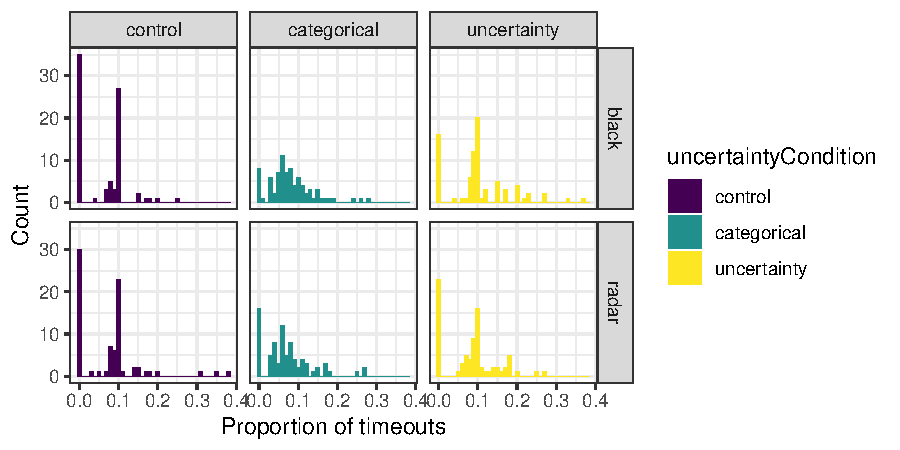
\includegraphics{images/DSTL08CLhistogramTimeouts}
	\caption{Proportion of timeouts in the category learning phase.}
	\label{fig:DSTL08CLhistogramTimeouts}
\end{figure}

\subsubsection{Trials to criterion.}
To judge learning speed, we looked at the number of trials it took for participants to reach the learning criterion (see Figure~\ref{fig:DSTL08CLboxplotTrialsCriterion}).
As the data violated assumptions of normality (Shapiro-Wilk, $W=0.66$, $p<.001$) and homogeneity of variance (Levene's Test, $F(5, 474)=11.96$, $p<.001$), we conducted a between-subjects ANOVA on the squared number of trials to criteria. 
We found that there was a significant main effect of uncertainty presentation conditions, $F(2, 474)=20.60$, $BF=1.63 \times 10^{17}$, $p<.001$. 
Looking at the pairwise comparisons with Tukey HSD, participants in the categorical conditions took significantly longer to learn than those in both the control ($p_{adj}<.001$) and uncertainty conditions ($p_{adj}<.001$). 
The difference between the control and uncertainty conditions was not significant ($p=.464$). 
There was not a main effect of background condition, $F(1, 474)=0.05$, $BF=0.11$,$p=.825$, where participants took longer to learn in the blue conditions than the green conditions. 
The interaction did not reach significance, $F(2,474)=0.18$, $BF=0.05$, $p=.839$. 

\begin{figure}[t!]
	\centering
	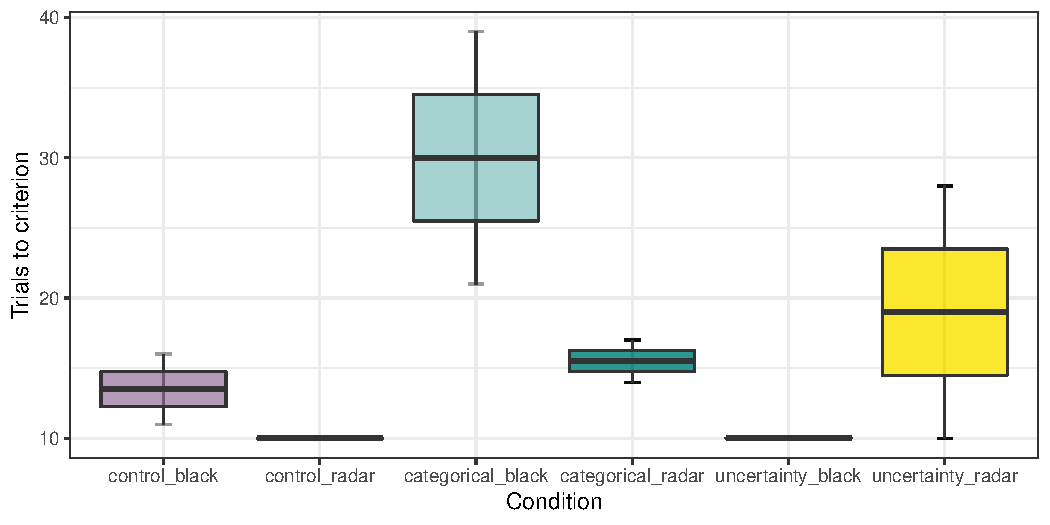
\includegraphics[width=\textwidth]{images/DSTL08CLboxplotTrialsCriterion}
	\caption{Number of trials to criterion in the category learning phase.}
	\label{fig:DSTL08CLboxplotTrialsCriterion}
\end{figure}

\subsubsection{Reaction time.}
Next, we looked at the reactions times (see Figure~\ref{fig:DSTL08CLboxplotRT}).
The data violated assumptions of normality (Shapiro-Wilk, $W=0.97$, $p<.001$), however, on inspection of the Q-Q plot the data appeared reasonably normal so we proceeded with untransformed data. 
We found a main effect of uncertainty presentation on reaction time, $F(2, 474)=38.83$, $BF=1.2\times 10^{13}$, $p<.001$. 
Looking at the pairwise comparisons with Tukey HSD, participants in the control conditions were faster to respond than those in the categorical ($p<.001$) and uncertainty ($p<.001$) conditions. 
The difference between categorical and uncertainty conditions also reached significance ($p=.013$).
The main effect of background did not reach significance, $F(1, 474)=0.69$,  $BF=0.13$, $p=.408$. 
However, the interaction did reach significance, $F(1, 474)=6.49$, $BF=14.87$, $p=.002$.

\begin{figure}[h!]
	\centering
	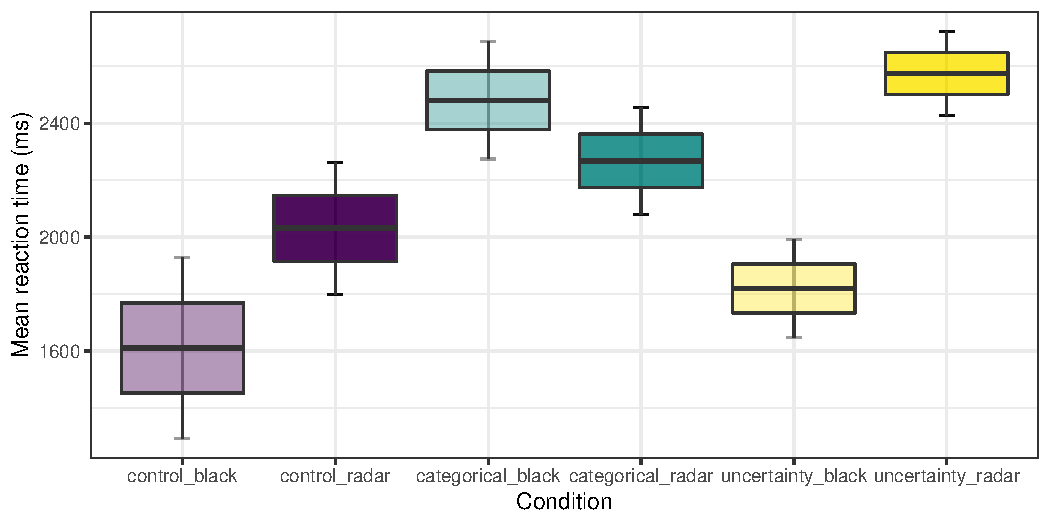
\includegraphics[width=\textwidth]{images/DSTL08CLboxplotRT.pdf}	
	\caption{Reaction time in the category learning phase.}
	\label{fig:DSTL08CLboxplotRT}
\end{figure}

\subsection{Change detection}
\subsubsection{Accuracy}
In this section, we report analyses examining the effect of uncertainty presentation on accuracy. 
Trials were defined as correct if on a change trial the participant clicked on the correct entity or if on a no change trial they withheld their response. 
The remaining trials were defined as incorrect. 

The distributions of participants' mean accuracies are shown in Figure~\ref{fig:DSTL08MboxplotAccuracy}. 
We defined outliers as those participants who scored lower than the first quartile minus 1.5 times the interquartile range or who scored greater than the third quartile plus 1.5 the interquartile range. 
This resulted in us excluding two participant from the control-radar condition. 

An ANOVA found a significant main effect of uncertainty presentation, $F(2,472)=101.27$, $BF_{10}=3.72 \times 10^{34}$, $p<.001$. 
Looking at the post-hoc pairwise comparisons, corrected using the Tukey method, we see that accuracy in the control condition, $M_\text{control}=0.27$, was significantly lower than the uncertainty condition, $M_\text{uncertainty}=0.53$, $t(472)=12.82$, $SE=0.02$, $p<.001$.
Similarly,  participants in the uncertainty conditions performed significantly better than those in the categorical conditions, $M_\text{categorical}=0.28$, $t(472)=12.37$, $SE=0.02$, $p<.001$. 
There was no significant difference between the control and categorical conditions,  $t(472)=0.48$, $SE=0.02$, $p=.879$. 
There was also a main effect of background, $F(1, 472)= 14.75$, $BF_{10}=12.58$, $p<.001$.
Participants were more accurate when the background was black, $M_\text{black}=0.39$, $SE=0.01$, than with the radar, $M_\text{radar}=0.33$, $SE=0.01$. 
The interaction between uncertainty presentation and colour did not reach significance, $F(2, 472)=0.28$, $BF_{10}=0.05$, $p=.756$. 

\begin{figure}[t!]
	\centering
	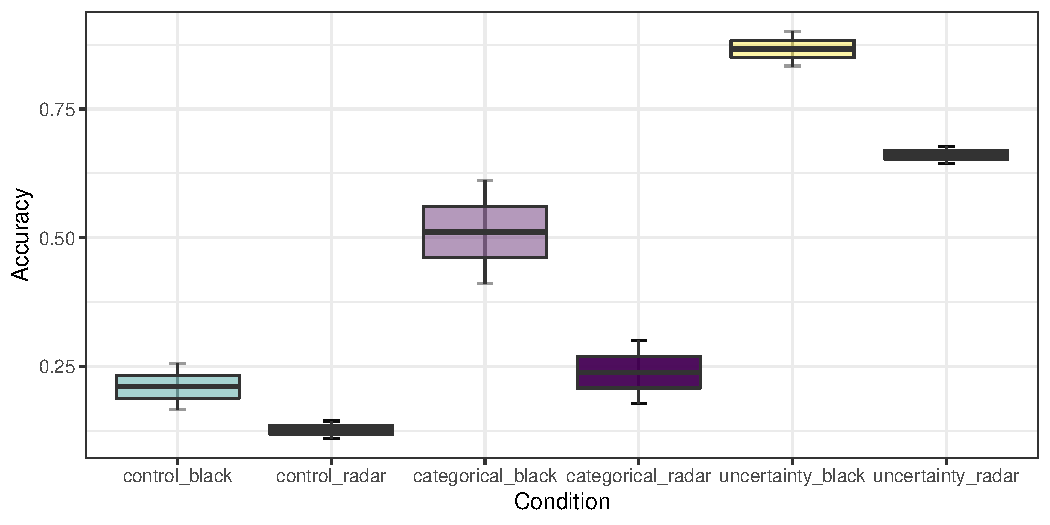
\includegraphics[width=\textwidth]{images/DSTL08MboxplotAccuracy}
	\caption{Boxplots of mean accuracy scores by conditions. }
	\label{fig:DSTL08MboxplotAccuracy}
\end{figure}

\subsubsection{Reaction time} 
Looking at timeouts, there were more timeouts in the control condition than the other conditions (see Figure~\ref{fig:DSTL08MboxplotTimeouts}).
Generally, participants had more timeouts in the control condition than than the other conditions. 

\begin{figure}[ht!]
	\centering
	\includegraphics[width=0.9\textwidth]{images/DSTL08MboxplotTimeouts}
	\caption{Boxplots of number of timeouts in the monitoring task across conditions.}
	\label{fig:DSTL08MboxplotTimeouts}
\end{figure}

The mean reaction times are shown in Figure~\ref{fig:DSTL03MboxplotRT}. 
We removed the outliers shown in the graph: two from the control-black condition, two from the control-radar, three from the categorical-radar, three from the uncertainty-black and three from the uncertainty-radar.  

An ANOVA found that the main effect of uncertainty presentation condition was significant, $F(2, 461)= 9.04$, $BF_{10}=105.05$, $p<.001$. 
Looking at the post-hoc pairwise comparisons, corrected using the Tukey method, we see that reaction time in the control condition, $M_\text{control}=1516ms$, was significantly slower than the uncertainty condition, $M_\text{uncertainty}=1383ms$, $t(461)=2.73$, $SE=49.0$, $p=.018$.
Similarly,  participants in the uncertainty conditions performed significantly faster than those in the categorical conditions, $M_\text{categorical}=1588ms$, $t(461)=4.20$, $SE=48.9$, $p<.001$. 
There was no significant difference between the control and categorical conditions,  $t(461)=1.47$, $SE=48.8$, $p=.309$. 
The main effect of background was not significant, $F(1, 461)=1.56$, $BF_{10}=0.21$, $p=.213$; 
nor the interaction, $F(2, 461)=0.80$, $BF_{10}=0.09$, $p=.448$. 

\begin{figure}[bh!]
	\centering	
	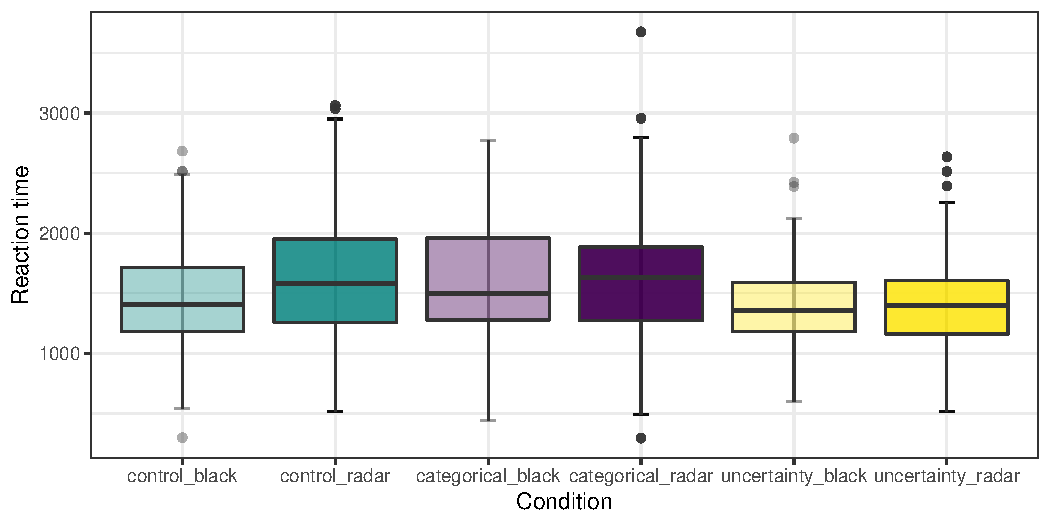
\includegraphics[width=\textwidth]{images/DSTL08MboxplotRT}
	\caption{Boxplots of mean reaction times by conditions.}
	\label{fig:DSTL08MboxplotRT}
\end{figure}

\clearpage
\newpage
\bibliographystyle{apacite}
\bibliography{references}

\end{document}
